%  Copyright (C) 2003 David Roundy
%
%  This program is free software; you can redistribute it and/or modify
%  it under the terms of the GNU General Public License as published by
%  the Free Software Foundation; either version 2, or (at your option)
%  any later version.
%
%  This program is distributed in the hope that it will be useful,
%  but WITHOUT ANY WARRANTY; without even the implied warranty of
%  MERCHANTABILITY or FITNESS FOR A PARTICULAR PURPOSE.  See the
%  GNU General Public License for more details.
%
%  You should have received a copy of the GNU General Public License
%  along with this program; if not, write to the Free Software Foundation,
%  Inc., 59 Temple Place - Suite 330, Boston, MA 02111-1307, USA.  
\documentclass[floats]{report}
\usepackage{color}
\usepackage{epsfig}
\usepackage{amsmath, amsthm, amssymb}

\usepackage{verbatim}
\usepackage{html}

\begin{document}

% Definition of title page:
\title{
    Dactyl\\
{\Large \it CYLindrical Time DomAin}
}
\author{
    David Roundy, Mihai Ibanescu, Peter Bermel
}

\maketitle 

\tableofcontents

\chapter{The Yee lattice}

\begin{figure}
\caption{Yee lattice in cylindrical coordinates.
\label{yee_fig}}
\centering
\mbox{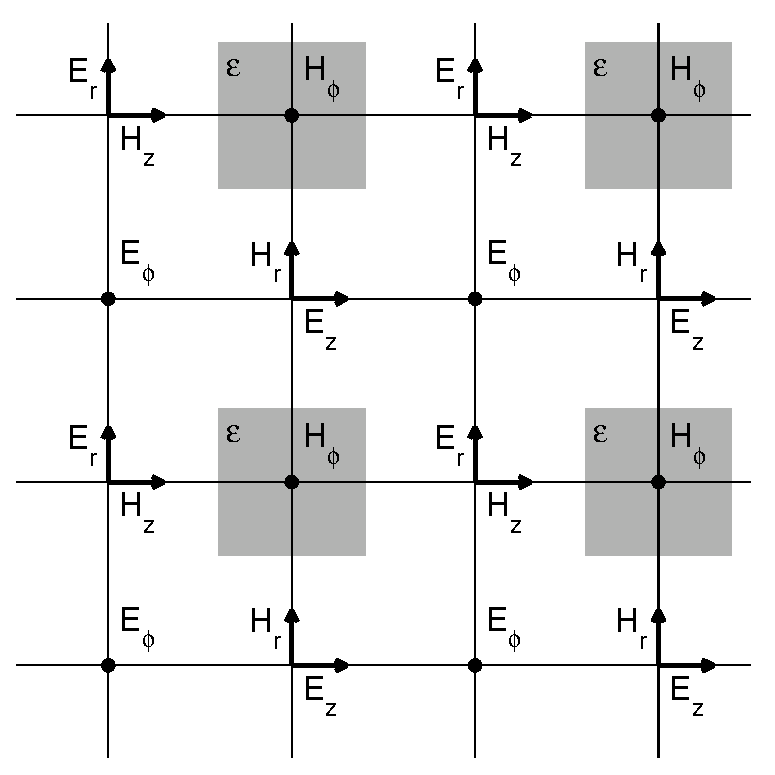
\epsfig{file=Yee_bulk.eps,width=7.8cm}}
\vspace{13cm}
\end{figure}

\chapter{Maxwell's equations in cylindrical coordinates}

Here are Maxwell's equations in cylindrical coordinates.  We take the
fields to be of the form:
\begin{equation*}
\mathbf{E}(r,\phi,z) = \mathbf{E}_m(r,z)e^{i m \phi} 
\end{equation*}

Without further ado:
\begin{align}
\frac1c\frac{dH_r}{dt} &= \frac{dE_\phi}{dz} - \frac{im}r E_z\\
\frac1c\frac{dH_\phi}{dt} &= \frac{dE_z}{dr} - \frac{dE_r}{dz}\\
\frac1c\frac{dH_z}{dt} &= \frac{im}r E_r - \frac1r\frac{d(rE_\phi)}{dr}
\end{align}
\begin{align}
\frac\epsilon c\frac{dE_r}{dt} &= \frac{im}r H_z - \frac{dH_\phi}{dz} \\
\frac\epsilon c\frac{dE_\phi}{dt} &= \frac{dH_r}{dz} - \frac{dH_z}{dr} \\
\frac\epsilon c\frac{dE_z}{dt} &= \frac1r\frac{d(rH_\phi)}{dr} - \frac{im}r H_r
\end{align}


\chapter{PML}

PML (Perfectly Matched Layers) is used to provide absorbing boundary
conditions in either the $z$ or $r$ direction.  PML consists of a material
in which some of the field components are split into two fields, each of
which has a conductivity associated with it, which is responsible for the
absorption of the PML.

PML is a sort of material that contains a set of conductivities $\sigma_r$,
$\sigma_\phi$ and $\sigma_z$.  These conductivities are both $\mathbf{E}$
and $\mathbf{H}$ conductivities---yes, we have magnetic monopoles moving
around in our PML.  $\ddot\smile$ Each $\sigma$ causes absorption of
radiation in the direction it is named after.  Thus $\sigma_\phi$ is small,
and almost unnecesary, and is only needed because of the curvature of the
radial surface.  The value of $\sigma_\phi$ at a given radius is equal to
\begin{equation}
\sigma_\phi(r) = \frac1r \int_0^r \sigma_r(r)dr
\end{equation}

If we had a IDTD (Infinitesimal Difference Time Domain) code, PML would be
perfectly absorbing, regardless of the variation of $\sigma$ with position.
However, since dactyl is a lowly FDTD code, we have to make sure that
$\sigma$ varies only slowly from one grid point to the next.  We do this by
making $\sigma_z$ (for example) vary as $z^2$, with a maximum value of
$\sigma_{max}$ right in front of the boundary.  At the edge of the PML
region is a metalic boundary condition.  The optimal value of
$\sigma_{max}$ is determined by a tradeoff between reflection off the
metallic boundary, caused by too little a $\sigma_{max}$, and reflection
off the sigma itself, caused by too large a $\sigma_{max}$, which makes for
a large variation of $\sigma$ from one grid point to the next.

Here are the field equations for a PML material:
\begin{align}
\frac{dH_{r\phi}}{dt} &= - c \frac{im}r E_z             - \sigma_\phi H_{r\phi} &
\frac{dH_{rz}}{dt} &= c \frac{dE_\phi}{dz}              - \sigma_z H_{rz}\\
\frac{dH_{\phi z}}{dt} &= - c \frac{dE_r}{dz}           - \sigma_z H_{\phi z} &
\frac{dH_{\phi r}}{dt} &= c \frac{dE_z}{dr}             - \sigma_r H_{\phi r} \\
\frac{dH_{zr}}{dt} &= - c \frac1r\frac{d(rE_\phi)}{dr}  - \sigma_r H_{zr}  &
\frac{dH_{z\phi}}{dt} &= c \frac{im}r E_r               - \sigma_\phi H_{z\phi} \\
\epsilon\frac{dE_{r\phi}}{dt} &=   c \frac{im}r H_z             - \sigma_\phi E_{r\phi} &
\epsilon\frac{dE_{rz}}{dt} &= -c\frac{dH_\phi}{dz}              - \sigma_z E_{rz}\\
\epsilon\frac{dE_{\phi z}}{dt} &=   c \frac{dH_r}{dz}           - \sigma_z E_{\phi z} &
\epsilon\frac{dE_{\phi r}}{dt} &=-c \frac{dH_z}{dr}             - \sigma_r E_{\phi r} \\
\epsilon\frac{dE_{zr}}{dt} &=   c \frac1r\frac{d(rH_\phi)}{dr}  - \sigma_r E_{zr}  &
\epsilon\frac{dE_{z\phi}}{dt} &=-c \frac{im}r H_r               - \sigma_\phi E_{z\phi} 
\end{align}

\chapter{Of polaritons and plasmons}\label{polaritons}

Most real materials, at least in some frequency range, have polarizations
that are not actually instantaneously proportional to the local electric
field.  We model these polaritonic and plasmonic effects by introducing one
or more additional polarization fields, to be propogated along with the
electric and magnetic field.  The polarization field, $\mathbf{P}$, is a
vector field which exists on the electric field Yee lattice points.

The polarization field obeys a second order differential equation, which
means that we need to keep track of the polarization at two time steps, in
order to integrate it.

\begin{equation}
\frac{d^2\mathbf{P}}{dt^2} + \gamma \frac{d\mathbf{P}}{dt}
+ \omega^2 \mathbf{P} = \Delta\epsilon\ \omega^2 \mathbf{E}
\end{equation}

To this, we need add one more term to maxwell's equation for $\mathbf E$:

\begin{equation}
c \nabla \times \mathbf{H} = \epsilon_\infty \frac{d\mathbf{E}}{dt}
 + \frac{d\mathbf{P}}{dt}
\end{equation}

So far, the polarization is beautifully simple.  However, we would love to
be able to put polaritonic materials into our PML regions, and
unfortunately in the PML region the electric field has been split into two
components, so we need to figure out which of the two components gets the
contribution from $\frac{d\mathbf{P}}{dt}$.  The obvious solution to this
(well, maybe not exactly obvious, but it is the solution) is to split the
polarization field also into two components in the PML region, just as we
split the electric and magnetic fields.

The electric field propogation equations in PML then become:
\begin{align}
\epsilon\frac{dE_{r\phi}}{dt} &=   c \frac{im}r H_z
             - \sigma_\phi E_{r\phi} - \frac{dP_{r\phi}}{dt} \\
\epsilon\frac{dE_{\phi z}}{dt} &=   c \frac{dH_r}{dz}
             - \sigma_z E_{\phi z} - \frac{dP_{\phi z}}{dt} \\
\epsilon\frac{dE_{zr}}{dt} &=   c \frac1r\frac{d(rH_\phi)}{dr}
             - \sigma_r E_{zr} - \frac{dP_{zr}}{dt}
\end{align}
\begin{align}
\epsilon\frac{dE_{rz}}{dt} &= -c\frac{dH_\phi}{dz}
             - \sigma_z E_{rz} - \frac{dP_{rz}}{dt}\\
\epsilon\frac{dE_{\phi r}}{dt} &=-c \frac{dH_z}{dr}
             - \sigma_r E_{\phi r} - \frac{dP_{\phi r}}{dt} \\
\epsilon\frac{dE_{z\phi}}{dt} &=-c \frac{im}r H_r \label{polariton_pml}
             - \sigma_\phi E_{z\phi} - \frac{dP_{z\phi}}{dt}
\end{align}

\chapter{Hints for writing finite difference time domain code}

(Or \emph{Things I forgot many times, so I wrote down so maybe I won't make
  the same mistake again.})

There is just one rule to remember when writing time domain code, and that
is (as Lefteris has repeatedly told me) ``Always know \emph{when} each
equation is evaluated.''  The trick, of course, lies in knowing how to
apply this rule, and remembering to actually apply it (and I think the
latter is perhaps harder than the former).

As an example, I'll convert a PML polariton equation into a finite
difference equation taken from equation~\ref{polariton_pml} of
chapter~\ref{polaritons}.
\begin{equation*}
\epsilon\frac{dE_{z\phi}}{dt} = -c \frac{im}r H_r
             - \sigma_\phi E_{z\phi} - \frac{dP_{z\phi}}{dt}
\end{equation*}
If we consider the $\mathbf{E}$ timesteps to be at times $n$, $n+1$ etc.,
then this equation needs to be evaluated at time $n+\frac12$.  This is no
problem for most of the terms, but it means that the $\sigma_\phi
E_{z\phi}$ term needs to be an average of its values at time $n$ and
$n+1$.  In short (taking $\Delta t$ to be unity)...
\begin{equation*}
\epsilon (E_{z\phi}^{n+1} - E_{z\phi}^n) = -c \frac{im}r H_r^{n+\frac12}
  - \sigma_\phi ( E_{z\phi}^{n+1} + E_{z\phi}^n) - (dP_{z\phi}^{n+1} - dP_{z\phi}^n)
\end{equation*}
Simplifying a tad gives
\begin{equation*}
E_{z\phi}^{n+1} - E_{z\phi}^n = \frac1{\epsilon + \frac12\sigma_\phi}
    \left(-c \frac{im}r H_r^{n+\frac12}
  - \sigma_\phi E_{z\phi}^n - (dP_{z\phi}^{n+1} - dP_{z\phi}^n)\right)
\end{equation*}
Basically, that is all there is to it.  You now have the equation to
determine $E_{z\phi}^{n+1}$ from $E_{z\phi}^n$, $\frac{im}r
H_r^{n+\frac12}$, $dP_{z\phi}^{n+1}$ and $dP_{z\phi}^n$.

\chapter{Tutorial}

\begin{comment}
/*
\end{comment}
\section{Baby's First Bandstructure}
\begin{comment}
*/
\end{comment}

\begin{comment}
#include <stdio.h>
#include <stdlib.h>
#include <meep.hpp>
using namespace meep;

double eps(const vec &) {
  return 1.0;
}
const int rad = 10;
const int ttot = 1500*rad;
\end{comment}

In this example we calculate the lowest four TE modes of a simple hollow
metallic waveguide of radius one.

\begin{verbatim}
int main(int argc, char *argv[]) {
  initialize mpi(argc, argv);
  FILE *ban = master_fopen("bands", "w");
  structure s(volcyl(1.0, 0.0, rad), eps);
  for (int m=0;m<3;m++) {
    for (double k=0.0; k<= 1.01; k += 0.25) {
      master_printf("Working on k of %g and m = %d with a=%d...\n",
                    k, m, rad);
      fields f(&s, m);
      f.use_bloch(k);
\end{verbatim}

There are a few tricks you should know before you decide to go about
calculating a band structure.  One of the biggest problems in calculating a
band structure in a time domain code is that of exciting all the modes you
are interested in.  Meep makes this easy with a couple of ``fields''
methods, \verb-initialize_with_n_te-, and \verb-initialize_with_n_tm-.
These initialize the field with the n lowest TE and TM modes respectively.

\begin{verbatim}
      f.initialize_with_n_te(4);
\end{verbatim}

The band structure code itself begins with a call to
\verb-prepare_for_bands-, which allocates space to store the field
data, which is later used for the band structure calculation.  Its third
argument is the maximum frequency you are interested in.

\begin{verbatim}
      double fmax = 1.0, qmin = 200;
      f.prepare_for_bands(0, ttot, fmax, qmin);
      for (int t=0;t<ttot;t++) {
\end{verbatim}

The second band structure function is \verb-record_bands-, which just
copies the fields into the already allocated arrays for future use.

\begin{verbatim}
        f.record_bands();
        f.step();
      }
\end{verbatim}

Finally, the band structure is actually computed and output by the method
\verb-output_bands-.  The key thing to know about
\verb-output_bands- is that its last argument should be something like
twice the number of modes which have a frequency below your maximum.
Rounding this number up slows the code down considerably, but can sometimes
fix problems where harminv (which is used internally) doesn't find the
modes correctly.  Usually, however, when harminv fails it means you are
misunderstanding something (for example, fmax may be less than the lowest
frequency mode).

\begin{verbatim}
      f.output_bands(ban, "band", 35);
    }
  }
  master_fclose(ban);
}
\end{verbatim}

\begin{comment}
#include <stdio.h>
#include <stdlib.h>

#include "dactyl.h"

const int a = 10;
\end{comment}

\section{Computing the band structure of an omniguide}

In this section we give as an example of a more complicated band structure,
a computation of the band structure of an omniguide.  The output of this
program is shown in Figure~\ref{omniguidebands}.

\begin{verbatim}
const int num_layers = 3;
const double rcore = 3.0;

double guided_eps(const vec &v) {
  double rr = v.r() - rcore;
  if (rr > num_layers + 0.3) return 1.0; // outside the entire waveguide
  if (rr < 0.0) return 1.0;   // vacuum in the core
  while (rr > 1.0) rr -= 1.0; // calculate (r - rcore) % 1
  if (rr < 0.3) return 21.16; // in the high dielectric
  return 1.6*1.6;             // in the low dielectric
}
\end{verbatim}

\begin{comment}
int main(int argc, char **argv) {
  deal_with_ctrl_c();
  printf("Running omniguide!\n");

  const double ttot = 1000.0;
  mat_chunk ma(volcyl(rcore + num_layers + 0.3, 0.0, a), guided_eps);
  const char *dirname = make_output_directory(argv[0]);
\end{comment}

For this band structure example, we use the grace object to create our
plot.
\begin{verbatim}
  grace g("bands", dirname);
  g.set_range(0.0, 0.35, 0.0, 0.35);
\end{verbatim}
\begin{comment}
  ma.set_output_directory(dirname);
  mat_chunk vac(&ma);
  vac.make_average_eps();
\end{comment}

Since the m = 0 modes are pure TE or TM, it makes sense to calculate the
two polarizations separately.  Not only does this give us more interesting
output, but it doesn't cost us any time, to speak of, and actually makes
the band structure much easier to converge.  However, for brevity, I won't
include here in the manual computation of the TM modes, but will skip
straight to the TE modes.

\begin{comment}
  {
    const int m=0;
    g.new_set();
    g.set_legend("m = 0, TM");
    for (double k=0.0;k<0.356 && !interrupt;k+=0.05) {
      char k_and_m[10];
      snprintf(k_and_m, 10, "%g-%d", k, m);
      printf("Working on k of %g and m=0 TM with a=%d...\n", k, a);
      fields_chunk f(&vac, m);
      f.use_bloch(k);
      f.verbose(1);
      f.phase_in_material(&ma, 1000);
      f.initialize_with_n_tm(9);
      double next_slice_time = 0.0;
      while (f.is_phasing() && !interrupt) {
        f.step();
      }
      f.prepare_for_bands(vec(4.801,0.0), ttot, .40, 300, 0.0);
      f.prepare_for_bands(vec(3.801,0.0), ttot, .40, 300, 0.0);
      f.prepare_for_bands(vec(3.301,0.0), ttot, .40, 300, 0.0);
      const double stoptime = f.time() + ttot;
      while (f.time() < stoptime && !interrupt) {
        f.record_bands();
        f.step();
      }
      f.grace_bands(&g, 40);
    }
  }
\end{comment}

\begin{figure}
\label{omniguidebands}
\caption{Omniguide band structure.}
\epsfig{file=omniguide-out/bands.eps,width=8.8cm}
\end{figure}

\begin{verbatim}
  for (int m=0;m<2 && !interrupt;m++) {
    g.new_set();
    char m_string[30];
    if (m) snprintf(m_string, 30, "m = %d", m);
    else snprintf(m_string, 30, "m = 0, TE");
    g.set_legend(m_string);
    for (double k=0.0;k<0.351 && !interrupt;k+=0.05) {
\end{verbatim}
\begin{comment}
      printf("Working on k of %g and %s with a=%d...\n", k, m_string, a);
      fields_chunk f(&vac, m);
      f.use_bloch(k);
      f.verbose(1);
      f.phase_in_material(&ma, 1000);
\end{comment}
We initialize the fields_chunk with both TE and TM modes, and then phase in the
epsilon as usual.
\begin{verbatim}
      f.initialize_with_n_te(9);
      if (m) f.initialize_with_n_tm(9);
\end{verbatim}
\begin{comment}
      while (f.is_phasing() && !interrupt) f.step();
\end{comment}
Again, the band structure code is pretty normal, with the only real
difference being that in this case we \emph{really} want to have specify a
large $Q_{min}$, to help dactyl to distinguish between real modes and
spurious noise.  Note that we are using metallic boundary conditions, so
all physical modes should have infinite lifetime.
\begin{verbatim}
      f.prepare_for_bands(vec(4.801,0.0), ttot, .35, 300, 0.0);
      f.prepare_for_bands(vec(1.801,0.0), ttot, .35, 300, 0.0);
      f.prepare_for_bands(vec(2.801,0.0), ttot, .35, 300, 0.0);
      const double stoptime = f.time() + ttot;
      while (f.time() < stoptime && !interrupt) {
        f.record_bands();
        f.step();
      }
\end{verbatim}
Finally, we just need to compute and output the bands.  We are careful here
to keep in mind that when $m > 0$, there are twice as many bands, since
there are both TM and TE modes.
\begin{verbatim}
      f.grace_bands(&g, m?80:40);
    }
\end{verbatim}
The band is actually printed to disk only when the grace object is
destroyed, which in this case happens just before the program exits.
\begin{comment}
  }
}
\end{comment}


\section{Band structure of a polariton}

\begin{comment}
#include <stdio.h>
#include <stdlib.h>

#include "dactyl.h"

const double rmax = 1.0;
\end{comment}

Here we compute and plot the band structure of a polariton material.  We
look at a simple metallic waveguide filled with a polaritonic material.
The material we look at has an epsilon of 13.4 and a longitudinal phonon
frequency of 0.7 and a transverse phonon frequency of 0.4.

\begin{figure}
\label{polaritonbands}
\caption{Polariton band structure.}
\epsfig{file=polaritonbands.eps,width=8.8cm}
\end{figure}

\begin{verbatim}
double eps(double r, double z) { return 13.4; }
double one(double r, double z) { return 1; }
\end{verbatim}

\begin{comment}
int main(int argc, char **argv) {
  deal_with_ctrl_c();
  const int a = 10;
  const int m = 0;
  double k;
  const int ttot = 1000*a;  
\end{comment}

\begin{comment}
  mat ma(eps, rmax, 0.0, a);
  const char *dirname = make_output_directory(argv[0]);
  printf("Storing output in directory %s/\n", dirname);
  FILE *ban = create_output_file(dirname, "bands");
  ma.set_output_directory(dirname);
\end{comment}

To create the polaritonic material, we add the polarizability to the
material after we have created it.

\begin{verbatim}
  double freq = 0.4, gamma = 0.01, delta_eps = 27.63;
  ma.add_polarizability(one, freq, gamma, delta_eps);
\end{verbatim}

\begin{verbatim}
  for (k=0.0;k<30.01 && !interrupt;k+=2.5) {
    printf("Working on k of %g and m = %d...\n", k, m);
    fields f(&ma, m);
    f.use_bloch(k);
\end{verbatim}

Now we excite the first TE mode (we are only looking at m = 0 here), and
remember to excite along with it the phonon with which it couples.

\begin{verbatim}
    f.initialize_with_nth_te(1);
    f.initialize_polarizations();
\end{verbatim}

Finally, we compute the band structure as usual.

\begin{verbatim}
    f.prepare_for_bands(0, ttot, .7+1.5*k/30.0, 40);
    
    for (int t=0; t < ttot+1 && !interrupt; t++) {
      f.record_bands();
      f.step();
    }
    f.output_bands(ban, "band", 16);
\end{verbatim}
\begin{comment}
    fflush(ban);
  }
  fclose(ban);
}
\end{comment}

The final output of this routine (as calculated using the ``plot'' program)
is shown in Figure~\ref{polaritonbands}.


\begin{comment}
#include <stdio.h>
#include <stdlib.h>
#include <signal.h>
\end{comment}

\section{Energy conservation in cylindrical coordinates}

In this example, we compute the total energy over time for a polaritonic
material in cylindrical coordinates.  Eventually I figure I may extend this
example to demonstrate energy/flux conservation using PML.  That would
definitely be more impressive.

\begin{figure}
\label{econs_cyl}
\caption{Energy vs. Time.}
\includegraphics[width=8.8cm,clip=true]{energy_cons-out/energy}
\end{figure}

\begin{comment}
#include <meep.hpp>
using namespace meep;

const double a = 10;
\end{comment}

For our example polaritonic material, we'll use an $\epsilon(0)$ of 13.4.
We will put the polaritons in just one quarter of our system to add a
little extra excitement.

\begin{verbatim}
double eps(const vec &) { return 13.4; }
double one(const vec &p) { return (p.z() > 15.0)?1:0; }
\end{verbatim}
\begin{comment}
int main(int argc, char **argv) {
  initialize mpi(argc, argv);
  deal_with_ctrl_c();
  const double ttot = 600.0;
\end{comment}
We use a long and skinny system so as to exaggerate any errors that may
crop up at small $r$.
\begin{verbatim}
  structure s(volcyl(1.0,20.0, a), eps);
\end{verbatim}
\begin{comment}
  const char *dirname = make_output_directory(__FILE__);
  s.set_output_directory(dirname);
  s.add_polarizability(one, 0.25, 0.1, 3.0);
  fields f(&s);
  grace g("energy", dirname);
\end{comment}
We use several point sources, to cover a broad frequency range, just for
the heck of it.
\begin{verbatim}
  f.add_point_source(Ep, 0.6 , 1.8, 0.0, 8.0, veccyl(0.5,2.0));
  f.add_point_source(Ep, 0.4 , 1.8, 0.0, 8.0, veccyl(0.5,2.0));
  f.add_point_source(Ep, 0.33, 1.8, 0.0, 8.0, veccyl(0.5,2.0));
\end{verbatim}
\begin{comment}
  double next_printtime = 50;
  while (f.time() < ttot && !interrupt) {
    if (f.time() >= next_printtime) {
      next_printtime += 50;
      master_printf("Working on time %g...  ", f.time());
      master_printf("energy is %g\n", f.total_energy());
\end{comment}
We plot the total energy, the electromagnetic energy and the
``thermodynamic energy'' which is the energy that is either stored in the
polarization, or has been converted into heat, or (if we had a saturating
gain system) perhaps is stored in a population inversion.
\begin{verbatim}
      g.output_out_of_order(0, f.time(), f.total_energy());
      g.output_out_of_order(1, f.time(), f.field_energy_in_box(f.v.surroundings()));
      g.output_out_of_order(2, f.time(), f.thermo_energy_in_box(f.v.surroundings()));
\end{verbatim}
\begin{comment}
    }
    f.step();
  }
}
\end{comment}


\begin{comment}
#include <stdio.h>
#include <stdlib.h>
#include <signal.h>
\end{comment}

\section{Energy conservation in one dimension}

In this example, we compute the total energy over time for a polaritonic
material in one dimension to verify that it is indeed conserved.  This also
demostrates how to use a 1D system.

\begin{figure}
\label{econs_1d}
\caption{Energy vs. Time.}
\epsfig{file=energy_cons_1d-out/energy.eps,width=8.8cm}
\end{figure}

\begin{comment}
#include "dactyl.h"

const int a = 10;
\end{comment}

For our example polaritonic material, we'll use an $\epsilon(0)$ of 13.4.

\begin{verbatim}
double eps(const vec &) { return 13.4; }
double one(const vec &) { return 1; }
\end{verbatim}
\begin{comment}
int main(int argc, char **argv) {
  deal_with_ctrl_c();
  const double ttot = 600.0;
\end{comment}
We create a 1D system by making the volume with the ``\verb!volone!''
function, and making sure any vecs we use are one dimensional.
\begin{verbatim}
  mat ma(volone(10.0, a), eps);
\end{verbatim}
\begin{comment}
  const char *dirname = make_output_directory(argv[0]);
  ma.set_output_directory(dirname);
\end{comment}
The polarizability is added as usual...
\begin{verbatim}
  ma.add_polarizability(one, 0.25, 0.01, 3.0);
  fields f(&ma);
  grace g("energy", dirname);
\end{verbatim}
We use several plane wave sources, to cover a broad frequency range, just
for the heck of it.
\begin{verbatim}
  f.add_point_source(Ex, 0.6 , 0.8, 0.0, 8.0, vec(2.0));
  f.add_point_source(Ex, 0.4 , 0.8, 0.0, 8.0, vec(2.0));
  f.add_point_source(Ex, 0.33, 0.8, 0.0, 8.0, vec(2.0));
\end{verbatim}
\begin{comment}
  double next_printtime = 10;
  while (f.time() < ttot && !interrupt) {
    if (f.time() >= next_printtime) {
      next_printtime += 10;
      printf("Working on time %lg...  ", f.time());
      printf("energy is %lg\n", f.total_energy());
      printf("magnetic energy is %lg\n", f.magnetic_energy_in_box(f.v));
      printf("electric energy is %lg\n", f.electric_energy_in_box(f.v));
      printf("thermo energy is %lg\n", f.thermo_energy_in_box(f.v));
\end{comment}
We plot the total energy, the electromagnetic energy and the
``thermodynamic energy'' which is the energy that is either stored in the
polarization, or has been converted into heat, or (if we had a saturating
gain system) perhaps is stored in a population inversion.
\begin{verbatim}
      g.output_out_of_order(0, f.time(), f.total_energy());
      g.output_out_of_order(1, f.time(),
                            f.electric_energy_in_box(f.v)
                          + f.magnetic_energy_in_box(f.v));
      g.output_out_of_order(2, f.time(),
                            f.thermo_energy_in_box(f.v));
\end{verbatim}
\begin{comment}
    }
    f.step();
  }
}
\end{comment}



\begin{comment}
#include <stdio.h>
#include <stdlib.h>
#include <signal.h>

#include "dactyl.h"
\end{comment}

\section{Epsilon of a polaritonic material in one dimension}

In this example, we compute epsilon as a function of frequency for a simple
polaritonic material.  This example is done in one dimension for speed
purposes.

One thing to be aware of when using polaritonic materials, is that
generally you will be needing a rather higher grid resolution than you may
be used to in order to properly model the material.  Here I am using an $a$
of 40.

\begin{figure}
\label{epsilon_polariton}
\caption{Epsilon of a polaritonic material.}
\epsfig{file=epsilon_polariton_1d-out/eps.eps,width=8.8cm}
\end{figure}


\begin{comment}
const double a = 10;
const double pml_thickness = 160.0/a;
const double middlesize = 5.0/a;
const double zsize = middlesize + 2*pml_thickness;
\end{verbatim}

For our example polaritonic material, we'll use an $\epsilon(0)$ of 13.4.

\begin{verbatim}
double eps(const vec &) { return 13.4; }
\end{verbatim}
\begin{comment}
double one_in_middle(const vec &p) {
  if (p.z() > pml_thickness && p.z() <= pml_thickness + middlesize) return 1;
  else return 0;
}

int main(int argc, char **argv) {
  deal_with_ctrl_c();
  const double ttot =1180.0;
  mat ma(volone(zsize, a), eps);
  const char *dirname = make_output_directory(argv[0]);
  ma.set_output_directory(dirname);
\end{comment}
Altough in this calculation the polaritonic material will not be within the
PML, it is all right to have polaritonic material within PML regions.
\begin{verbatim}
  ma.use_pml_right(pml_thickness);
  ma.use_pml_left(pml_thickness);
  ma.add_polarizability(one_in_middle, 0.4, 0.01, 27.63);
\end{verbatim}
\begin{comment}
  fields f(&ma);
  double sourceloc = pml_thickness+1.0/(double)a;
\end{comment}
We use a single rather high frequency (and very broad) point source, to
cover a broad frequency range.
\begin{verbatim}
  f.add_point_source(Ex, 0.9, 0.8, 0.0, 8.0, vec(sourceloc));
\end{verbatim}
We use a couple of monitor points to determine epsilon.
\begin{verbatim}
  monitor_point *left = NULL, *right = NULL, *middle = NULL;
\end{verbatim}
\begin{comment}
  double next_printtime = 50;
  while (f.time() < ttot && !interrupt) {
    if (f.time() >= next_printtime) {
      next_printtime += 50;
      printf("Working on time %lg...  ", f.time());
      printf("energy is %lg\n", f.field_energy());
    }
\end{comment}
The monitor points are located one grid spacing from one another.  The
\verb*|get_new_point| method appends the fields at a given time to a
monitor point linked list.
\begin{verbatim}
    left  = f.get_new_point(vec(sourceloc+1.0/a), left );
    middle = f.get_new_point(vec(sourceloc+2.0/a), middle);
    right = f.get_new_point(vec(sourceloc+3.0/a), right);
\end{verbatim}
\begin{comment}
    f.step();
  }
  grace g("eps", dirname);
  complex<double> *al, *ar, *am, *freqs;
  int numl, numr;
  printf("Working on left fourier transform...\n");
\end{comment}
When the time stepping is over, we take a fourier transform of the fields
at the two monitor points.
\begin{verbatim}
  left->fourier_transform(Ex, &al, &freqs, &numl, 0.301, 0.5, 300);
\end{verbatim}
\begin{comment}
  delete[] freqs;
  printf("Working on middle fourier transform...\n");
  middle->fourier_transform(Ex, &am, &freqs, &numr, 0.301, 0.5, 300);
  delete[] freqs;
  printf("Working on right fourier transform...\n");
  right->fourier_transform(Ex, &ar, &freqs, &numr, 0.301, 0.5, 300);
  if (numl != numr) printf("Aaack you need both nums to be the same!\n");
  g.new_set();
  g.set_legend("\\x\\e\\s1\\N");
\end{comment}
Finally we calculate epsilon from the second derivative of the field using
\begin{equation*}
-k^2 H_z(\omega) = \nabla^2 H_z(\omega) = \nabla^2
\end{equation*}
\begin{verbatim}
  complex<double> *epsilon = new complex<double>[numl];
  for (int i=0;i<numl;i++) {
    complex<double> ksqr = -(ar[i]+al[i]-2*am[i])*a*a/am[i];
    epsilon[i] = ksqr/freqs[i]/freqs[i]/(2*pi*2*pi);
  } 
  for (int i=0;i<numl;i++)
    g.output_point(real(freqs[i]), real(epsilon[i]));
  g.new_set();
  g.set_legend("\\x\\e\\s2\\N");
  for (int i=0;i<numl;i++)
    g.output_point(real(freqs[i]), imag(epsilon[i]));
\end{verbatim}
\begin{comment}
  g.new_set();
  g.set_legend("analytic \\x\\e\\s1\\N");
  for (int i=0;i<numl;i++) {
    g.output_point(real(freqs[i]),
                   real(f.analytic_epsilon(real(freqs[i]),vec(sourceloc+3.0/a))));
  }
  g.new_set();
  g.set_legend("analytic \\x\\e\\s2\\N");
  for (int i=0;i<numl;i++) {
    g.output_point(real(freqs[i]),
                   imag(f.analytic_epsilon(real(freqs[i]),vec(sourceloc+3.0/a))));
  }
}
\end{comment}



\section{Dielectric function of a material with loss and gain}

\begin{comment}
#include <stdio.h>
#include <stdlib.h>
#include <signal.h>

#include "dactyl.h"

const int a = 10;
const int m = 0;
const double eps_value = 2.25;
const double fmin = 0.05;

const double pml = 1.0;
const int npml = (int)(0.5+pml*a);
const double zsize = 2*pml+10/(double)a;//+1.0/freq;
const double rmax  = 6/(double)a;
const double zmiddle = zsize/2;
const double sourceloc = zmiddle - 4/(double)a;

const double r_look = 1.5/a, z_look = zmiddle, d = 1.0/a;

double eps(const vec &) { return eps_value; }
double one_in_middle(const vec &v) {
  const double midmax = r_look+2.0/(double)a;
  const double midwid = 2/(double)a;
  if (v.r() <= midmax && v.z() >= zmiddle-midwid && v.z() < zmiddle+midwid) {
    return 1;
  } else {
    return 0;
  }
}

int main(int argc, char **argv) {
  deal_with_ctrl_c();
  const char *dirname = make_output_directory(argv[0]);
  printf("Using pml of %lg thickness.\n", pml);
  printf("Using an rmax of %lg\n", rmax);
  mat ma(volcyl(rmax + pml, zsize, a), eps);
  ma.use_pml_right(pml);
  ma.use_pml_left(pml);
  ma.use_pml_radial(pml);
  ma.set_output_directory(dirname);
\end{comment}

In this section, we demonstrate a better way to calculate the dielectric
function, and illustrate it by computing the dielectric function of a
material with a normal lossy resonance as well as a gain line.  Gain in the
PML is a bad idea, so we restrict the polarizabilities to exist only in the
middle of the system (which is surrounded by PML).

\begin{figure}
\label{lossgain_epsilon}
\caption{Dielectric function of a material with loss and gain.}
\epsfig{file=lossgain_epsilon-out/eps.eps,width=8.8cm}
\end{figure}

\begin{verbatim}
  ma.add_polarizability(one_in_middle, 0.195, 0.03, 0.25*.25/.195);
  ma.add_polarizability(one_in_middle, 0.25, 0.03,-0.25);
\end{verbatim}

\begin{comment}
  ma.output_slices();

  fields f(&ma, m);
\end{comment}

For sources, we use a series of broad point sources covering the frequency
range of interest.

\begin{verbatim}
  f.add_point_source(Ep, 0.9, 0.8, 0.0, 8.0, vec(rmax*.5,sourceloc));
\end{verbatim}
\begin{comment}
  printf("Working with a=%d...\n", a);
  monitor_point *left = NULL, *right = NULL, *middle = NULL,
                *top = NULL, *bottom = NULL;
  double next_printtime = 10;
  while (f.time() < 130 && !interrupt) {
    if (f.time() >= next_printtime) {
      next_printtime += 10;
      printf("Working on time %lg...  ", f.time());
      printf("energy is %lg\n", f.field_energy());
      //if (f.time() > -90) f.eps_slices();
    }
    f.step();
\end{comment}

The calculation proceeds as usual, except that we now keep track of a set
of monitor points that will allow us to take a laplacian of the $H_z$ field
component.  We choose $m=0$, so we won't have to deal with the $\phi$
derivative.

\begin{verbatim}
    left   = f.get_new_point(vec(r_look    , z_look - d), left);
    middle = f.get_new_point(vec(r_look    , z_look    ), middle);
    top    = f.get_new_point(vec(r_look + d, z_look    ), top);
    bottom = f.get_new_point(vec(r_look - d, z_look    ), bottom);
    right  = f.get_new_point(vec(r_look    , z_look + d), right);
\end{verbatim}
\begin{comment}
  }

  grace g("eps", dirname);
  complex<double> *al, *ar, *am, *at, *ab, *freqs;
  int numl, numr;
  printf("Working on left fourier transform...\n");
\end{comment}

We fourier transform $H_z$ at each point:

\begin{verbatim}
  left->fourier_transform(Hz, &al, &freqs, &numl, 0.101, 0.5, 1000);
\end{verbatim}
\begin{comment}
  delete[] freqs;
  printf("Working on middle fourier transform...\n");
  middle->fourier_transform(Hz, &am, &freqs, &numr, 0.101, 0.5, 1000);
  delete[] freqs;
  printf("Working on top fourier transform...\n");
  top->fourier_transform(Hz, &at, &freqs, &numr, 0.101, 0.5, 1000);
  delete[] freqs;
  printf("Working on bottom fourier transform...\n");
  bottom->fourier_transform(Hz, &ab, &freqs, &numr, 0.101, 0.5, 1000);
  delete[] freqs;
  printf("Working on right fourier transform...\n");
  right->fourier_transform(Hz, &ar, &freqs, &numr, 0.101, 0.5, 1000);
  if (numl != numr) printf("Aaack you need both nums to be the same!\n");
  g.new_set();
  g.set_legend("\\x\\e\\s1\\N");
  complex<double> *epsilon = new complex<double>[numl];
\end{comment}

Finally, we calculate the laplacian of $H_z(\omega)$, which is equal to
$-k^2 H_z(\omega)$, from which we extract epsilon.

\begin{verbatim}
  for (int i=0;i<numl;i++) {
    complex<double> ksqr = -(ar[i]+al[i]-2*am[i]
                             + at[i]+ab[i]-2*am[i]
                             + (at[i]-ab[i])/2/r_look/a
                             )*a*a/am[i];
    epsilon[i] = ksqr/freqs[i]/freqs[i]/(2*pi*2*pi);
  }
\end{verbatim}

I've left out the bulk of this example from the manual itself, since it
is pretty much the same as the previous examples.  Among other features, we
use the grace functions to plot the result, which can be seen in
Figure~\ref{lossgain_epsilon}.

\begin{comment}
  for (int i=0;i<numl;i++) {
    g.output_point(real(freqs[i]), real(epsilon[i]));
  }
  g.new_set();
  g.set_legend("\\x\\e\\s2\\N");
  for (int i=0;i<numl;i++) {
    g.output_point(real(freqs[i]), imag(epsilon[i]));
  }
}
\end{comment}


\appendix

% This is the FSF GPL, translated to LaTeX by David Roundy

\chapter{GNU General Public License}
\label{gpl}
\section*{Version 2, June 1991}

% This file is intended to be included in another file.

\newcommand{\myhead}[1]{{\Large\begin{center}#1\end{center}}}

\begin{quote}
Copyright \copyright\ 1989, 1991 Free Software Foundation, Inc.\\
59 Temple Place - Suite 330, Boston, MA  02111-1307, USA

Everyone is permitted to copy and distribute verbatim copies
of this license document, but changing it is not allowed.
\end{quote}

\section*{Preamble}

  The licenses for most software are designed to take away your
freedom to share and change it.  By contrast, the GNU General Public
License is intended to guarantee your freedom to share and change free
software---to make sure the software is free for all its users.  This
General Public License applies to most of the Free Software
Foundation's software and to any other program whose authors commit to
using it.  (Some other Free Software Foundation software is covered by
the GNU Library General Public License instead.)  You can apply it to
your programs, too.

  When we speak of free software, we are referring to freedom, not
price.  Our General Public Licenses are designed to make sure that you
have the freedom to distribute copies of free software (and charge for
this service if you wish), that you receive source code or can get it
if you want it, that you can change the software or use pieces of it
in new free programs; and that you know you can do these things.

  To protect your rights, we need to make restrictions that forbid
anyone to deny you these rights or to ask you to surrender the rights.
These restrictions translate to certain responsibilities for you if you
distribute copies of the software, or if you modify it.

  For example, if you distribute copies of such a program, whether
gratis or for a fee, you must give the recipients all the rights that
you have.  You must make sure that they, too, receive or can get the
source code.  And you must show them these terms so they know their
rights.

  We protect your rights with two steps: (1) copyright the software, and
(2) offer you this license which gives you legal permission to copy,
distribute and/or modify the software.

  Also, for each author's protection and ours, we want to make certain
that everyone understands that there is no warranty for this free
software.  If the software is modified by someone else and passed on, we
want its recipients to know that what they have is not the original, so
that any problems introduced by others will not reflect on the original
authors' reputations.

  Finally, any free program is threatened constantly by software
patents.  We wish to avoid the danger that redistributors of a free
program will individually obtain patent licenses, in effect making the
program proprietary.  To prevent this, we have made it clear that any
patent must be licensed for everyone's free use or not licensed at all.

  The precise terms and conditions for copying, distribution and
modification follow.

\myhead{GNU GENERAL PUBLIC LICENSE}
\myhead{TERMS AND CONDITIONS FOR COPYING, DISTRIBUTION AND MODIFICATION}

\begin{enumerate} % Should start at zero here...
\setcounter{enumi}{-1}
\item
This License applies to any program or other work which contains
a notice placed by the copyright holder saying it may be distributed
under the terms of this General Public License.  The ``Program'', below,
refers to any such program or work, and a ``work based on the Program''
means either the Program or any derivative work under copyright law:
that is to say, a work containing the Program or a portion of it,
either verbatim or with modifications and/or translated into another
language.  (Hereinafter, translation is included without limitation in
the term ``modification''.)  Each licensee is addressed as ``you''.

Activities other than copying, distribution and modification are not
covered by this License; they are outside its scope.  The act of
running the Program is not restricted, and the output from the Program
is covered only if its contents constitute a work based on the
Program (independent of having been made by running the Program).
Whether that is true depends on what the Program does.

\item
You may copy and distribute verbatim copies of the Program's
source code as you receive it, in any medium, provided that you
conspicuously and appropriately publish on each copy an appropriate
copyright notice and disclaimer of warranty; keep intact all the
notices that refer to this License and to the absence of any warranty;
and give any other recipients of the Program a copy of this License
along with the Program.

You may charge a fee for the physical act of transferring a copy, and
you may at your option offer warranty protection in exchange for a fee.

\item
You may modify your copy or copies of the Program or any portion
of it, thus forming a work based on the Program, and copy and
distribute such modifications or work under the terms of Section 1
above, provided that you also meet all of these conditions:

\begin{enumerate} % Starting with a
\item
You must cause the modified files to carry prominent notices
stating that you changed the files and the date of any change.

\item
You must cause any work that you distribute or publish, that in
whole or in part contains or is derived from the Program or any
part thereof, to be licensed as a whole at no charge to all third
parties under the terms of this License.

\item
If the modified program normally reads commands interactively
when run, you must cause it, when started running for such
interactive use in the most ordinary way, to print or display an
announcement including an appropriate copyright notice and a
notice that there is no warranty (or else, saying that you provide
a warranty) and that users may redistribute the program under
these conditions, and telling the user how to view a copy of this
License.  (Exception: if the Program itself is interactive but
does not normally print such an announcement, your work based on
the Program is not required to print an announcement.)
\end{enumerate}

These requirements apply to the modified work as a whole.  If
identifiable sections of that work are not derived from the Program,
and can be reasonably considered independent and separate works in
themselves, then this License, and its terms, do not apply to those
sections when you distribute them as separate works.  But when you
distribute the same sections as part of a whole which is a work based
on the Program, the distribution of the whole must be on the terms of
this License, whose permissions for other licensees extend to the
entire whole, and thus to each and every part regardless of who wrote it.

Thus, it is not the intent of this section to claim rights or contest
your rights to work written entirely by you; rather, the intent is to
exercise the right to control the distribution of derivative or
collective works based on the Program.

In addition, mere aggregation of another work not based on the Program
with the Program (or with a work based on the Program) on a volume of
a storage or distribution medium does not bring the other work under
the scope of this License.

\item
You may copy and distribute the Program (or a work based on it,
under Section 2) in object code or executable form under the terms of
Sections 1 and 2 above provided that you also do one of the following:

\begin{enumerate} % Starting with a
\item
Accompany it with the complete corresponding machine-readable
source code, which must be distributed under the terms of Sections
1 and 2 above on a medium customarily used for software interchange; or,

\item
Accompany it with a written offer, valid for at least three
years, to give any third party, for a charge no more than your
cost of physically performing source distribution, a complete
machine-readable copy of the corresponding source code, to be
distributed under the terms of Sections 1 and 2 above on a medium
customarily used for software interchange; or,

\item
Accompany it with the information you received as to the offer
to distribute corresponding source code.  (This alternative is
allowed only for noncommercial distribution and only if you
received the program in object code or executable form with such
an offer, in accord with Subsection b above.)
\end{enumerate}

The source code for a work means the preferred form of the work for
making modifications to it.  For an executable work, complete source
code means all the source code for all modules it contains, plus any
associated interface definition files, plus the scripts used to
control compilation and installation of the executable.  However, as a
special exception, the source code distributed need not include
anything that is normally distributed (in either source or binary
form) with the major components (compiler, kernel, and so on) of the
operating system on which the executable runs, unless that component
itself accompanies the executable.

If distribution of executable or object code is made by offering
access to copy from a designated place, then offering equivalent
access to copy the source code from the same place counts as
distribution of the source code, even though third parties are not
compelled to copy the source along with the object code.

\item
You may not copy, modify, sublicense, or distribute the Program
except as expressly provided under this License.  Any attempt
otherwise to copy, modify, sublicense or distribute the Program is
void, and will automatically terminate your rights under this License.
However, parties who have received copies, or rights, from you under
this License will not have their licenses terminated so long as such
parties remain in full compliance.

\item
You are not required to accept this License, since you have not
signed it.  However, nothing else grants you permission to modify or
distribute the Program or its derivative works.  These actions are
prohibited by law if you do not accept this License.  Therefore, by
modifying or distributing the Program (or any work based on the
Program), you indicate your acceptance of this License to do so, and
all its terms and conditions for copying, distributing or modifying
the Program or works based on it.

\item
Each time you redistribute the Program (or any work based on the
Program), the recipient automatically receives a license from the
original licensor to copy, distribute or modify the Program subject to
these terms and conditions.  You may not impose any further
restrictions on the recipients' exercise of the rights granted herein.
You are not responsible for enforcing compliance by third parties to
this License.

\item
If, as a consequence of a court judgment or allegation of patent
infringement or for any other reason (not limited to patent issues),
conditions are imposed on you (whether by court order, agreement or
otherwise) that contradict the conditions of this License, they do not
excuse you from the conditions of this License.  If you cannot
distribute so as to satisfy simultaneously your obligations under this
License and any other pertinent obligations, then as a consequence you
may not distribute the Program at all.  For example, if a patent
license would not permit royalty-free redistribution of the Program by
all those who receive copies directly or indirectly through you, then
the only way you could satisfy both it and this License would be to
refrain entirely from distribution of the Program.

If any portion of this section is held invalid or unenforceable under
any particular circumstance, the balance of the section is intended to
apply and the section as a whole is intended to apply in other
circumstances.

It is not the purpose of this section to induce you to infringe any
patents or other property right claims or to contest validity of any
such claims; this section has the sole purpose of protecting the
integrity of the free software distribution system, which is
implemented by public license practices.  Many people have made
generous contributions to the wide range of software distributed
through that system in reliance on consistent application of that
system; it is up to the author/donor to decide if he or she is willing
to distribute software through any other system and a licensee cannot
impose that choice.

This section is intended to make thoroughly clear what is believed to
be a consequence of the rest of this License.

\item
If the distribution and/or use of the Program is restricted in
certain countries either by patents or by copyrighted interfaces, the
original copyright holder who places the Program under this License
may add an explicit geographical distribution limitation excluding
those countries, so that distribution is permitted only in or among
countries not thus excluded.  In such case, this License incorporates
the limitation as if written in the body of this License.

\item
The Free Software Foundation may publish revised and/or new versions
of the General Public License from time to time.  Such new versions will
be similar in spirit to the present version, but may differ in detail to
address new problems or concerns.

Each version is given a distinguishing version number.  If the Program
specifies a version number of this License which applies to it and ``any
later version'', you have the option of following the terms and conditions
either of that version or of any later version published by the Free
Software Foundation.  If the Program does not specify a version number of
this License, you may choose any version ever published by the Free Software
Foundation.

\item
If you wish to incorporate parts of the Program into other free
programs whose distribution conditions are different, write to the author
to ask for permission.  For software which is copyrighted by the Free
Software Foundation, write to the Free Software Foundation; we sometimes
make exceptions for this.  Our decision will be guided by the two goals
of preserving the free status of all derivatives of our free software and
of promoting the sharing and reuse of software generally.

\myhead{NO WARRANTY}

\item
BECAUSE THE PROGRAM IS LICENSED FREE OF CHARGE, THERE IS NO WARRANTY
FOR THE PROGRAM, TO THE EXTENT PERMITTED BY APPLICABLE LAW.  EXCEPT WHEN
OTHERWISE STATED IN WRITING THE COPYRIGHT HOLDERS AND/OR OTHER PARTIES
PROVIDE THE PROGRAM ``AS IS'' WITHOUT WARRANTY OF ANY KIND, EITHER EXPRESSED
OR IMPLIED, INCLUDING, BUT NOT LIMITED TO, THE IMPLIED WARRANTIES OF
MERCHANTABILITY AND FITNESS FOR A PARTICULAR PURPOSE.  THE ENTIRE RISK AS
TO THE QUALITY AND PERFORMANCE OF THE PROGRAM IS WITH YOU.  SHOULD THE
PROGRAM PROVE DEFECTIVE, YOU ASSUME THE COST OF ALL NECESSARY SERVICING,
REPAIR OR CORRECTION.

\item
IN NO EVENT UNLESS REQUIRED BY APPLICABLE LAW OR AGREED TO IN WRITING
WILL ANY COPYRIGHT HOLDER, OR ANY OTHER PARTY WHO MAY MODIFY AND/OR
REDISTRIBUTE THE PROGRAM AS PERMITTED ABOVE, BE LIABLE TO YOU FOR DAMAGES,
INCLUDING ANY GENERAL, SPECIAL, INCIDENTAL OR CONSEQUENTIAL DAMAGES ARISING
OUT OF THE USE OR INABILITY TO USE THE PROGRAM (INCLUDING BUT NOT LIMITED
TO LOSS OF DATA OR DATA BEING RENDERED INACCURATE OR LOSSES SUSTAINED BY
YOU OR THIRD PARTIES OR A FAILURE OF THE PROGRAM TO OPERATE WITH ANY OTHER
PROGRAMS), EVEN IF SUCH HOLDER OR OTHER PARTY HAS BEEN ADVISED OF THE
POSSIBILITY OF SUCH DAMAGES.
\end{enumerate}

\myhead{END OF TERMS AND CONDITIONS}

\end{document}

